\chapter{Hierarchical Clustering of LC-MS Peaks}
\label{c:hdp}

\section{Introduction}

The goal of establishing the matching of peaks across multiple runs at once can be viewed as a clustering problem, where a set of peaks can be grouped (by their m/z, RT and other suitable features) into local clusters within each run (representing all of the peaks from an individual compound), which are further grouped into global clusters shared across runs. A preliminary form of this idea has been explored in \cite{DeSouza2006}, where hierarchical clustering is performed on the total ion chromatogram data to group peaks into within-run local clusters, which are further grouped into across-run super clusters. The highly accurate mass information available from modern LC-MS platforms is not used in \cite{DeSouza2006}, although it is highlighted as a possible future work. The choice of using a hierarchical clustering method in \cite{DeSouza2006} also requires choosing various user-defined parameters, such as determining a suitable cut-off for the dendogram produced, deciding on a suitable linkage method and defining an appropriate distance measure between groups of peaks.

According to \cite{Smith2013}, the common shortcomings shared by many alignment methods include the incorrect modelling assumption that elution order of peaks is preserved across runs and the abundance of user-defined parameters, which can dramatically influence alignment results. Further uncertainties can be introduced due to the selection of a reference run and the construction of a guide tree in hierarchical methods. Since alignment is such an important part of the data preprocessing steps, it would be useful to be able to robustly identify the uncertainty or confidence in the alignment results. The subject of identifying and quantifying uncertainty has been extensively investigated in the problem of multiple sequence alignment (MSA) for genomics and transcriptomics. \cite{Landan2009} attempt to quantify the alignment uncertainty of the popular MSA tool ClustalW \cite{Thompson1994}, based on evaluations using synthetic data, and concludes that between half to all columns in their benchmark MSA results contain alignment errors. \cite{Notredame2000} construct a score that reflects the consensus between all possible pairwise alignments in T-COFFEE, while \cite{Penn2010} propose GUIDANCE, a confidence measure obtained from pertubations of guide trees. Statistical approaches that provide a measure of confidence in alignment results have also been explored by \cite{Redelings2005} and \cite{Bradley2009}, where the MSA results and phylogeny are constructed simultaneously, thus eliminating the need for a guide tree. 

Additionally, it is also desirable for alignment methods to provide some measure of confidence in the quality of its alignment. In the absence of ground truth information, the user typically measures alignment quality through manual inspection or by comparing and visualising the summary statistics (e.g. median, standard deviation of retention time) across different replicates. Alignment methods with confidence values is a big research gap that, to our knowledge, has not been addressed at all by any of the alignment tools surveyed earlier. Some interactive analysis tools like MAVEN \cite{Melamud2010} can assign quality scores to individual peaks. This is accomplished by training a neural network (or a decision tree) on training data that have been manually annotated using metrics of peak quality. Other approach like \cite{Brodsky2010} computes the Pearson correlations between intensity profiles of all peaks across replicates. Moving from these approaches towards a robust method that can provide confidence values for groups of aligned peaks across many label-free experiments is challenging research problem.

Despite the clear benefits of alignment uncertainty quantification in the sequence domain, the challenge of quantifying alignment results remains relatively unaddressed for the alignment of multiple runs in LC-MS-based-omics. Bayesian methods operating on profile data (e.g. \cite{Listgarten2004, Kong2009, Tsai2013a}) and feature-based alignment methods (e.g. \cite{Fischer2006, Pluskal2010, Voss2011a}) exist to correct RT drift, but in such methods, uncertainties are not propagated from the RT regression stage to the necessary peak matching stage that follows. Several recent feature-based alignment methods incorporate probabilistic modelling as part of their workflow, making it possible to extract some form of scores or probabilities on the alignment results. These methods are often limited to the alignment of two runs, which is not a realistic assumption in actual LC-MS experiments. For example, \cite{Jeong2012} propose an empirical Bayes model for pairwise peak matching. Matching confidence can be obtained from the model in form of posterior probability for any peak pair in two runs, however constructing multiple alignment results in \cite{Jeong2012} still requires a greedy search to find candidate features within m/z and RT-RT tolerances to a predetermined set of `landmark' peaks. \cite{GhanatBari2014b} describe PeakLink, a workflow for alignment that performs an initial warping using a fourth-degree polynomial. PeakLink poses the pairwise matching problem as a binary classification problem, where a Support Vector Machine (SVM) is trained based on an alignment ground truth derived from MS-MS information and used to differentiate matching and non-matching candidate pairs to produce the actual alignment results. While not explicitly included in the output of PeakLink, a matching score can be extracted from the SVM that represents how far each candidate pair is from the decision boundary. Note that these scores are not well-calibrated in the probabilistic sense, thus making comparisons of matching scores less straightforward. PeakLink is also not extended to the problem of aligning multiple runs, although \cite{GhanatBari2014b} state that it would be possible to do so with the choice of a suitable reference run.

In this work, we expand upon the idea of viewing direct matching as a hierarchical clustering problem by proposing \textbf{HDP-Align}, a Bayesian non-parametric model that groups related-peaks within runs and assigns them to global clusters shared across runs. Within each global cluster, peaks are further grouped by their m/z values into mass clusters, which represent the various ionisation products (IPs) derived from the global compound. The proposed model allows us to infer the matching of peaks across all runs at once, without the need for any intermediate merging of pairwise runs, and the resulting posterior summaries provide us with a confidence score in the matching quality of aligned peaksets. This introduces the possibility of allowing the user to trade recall for precision from the alignment results by returning a smaller subset of the results having a higher confidence score of being correctly aligned. Figure \ref{fig-hdp-cartoon} shows an illustration of the clustering process in HDP-Align. Additionally, the latent variables of clustering structure inferred in the model can potentially have physically meaningful identities that can be used for further analysis, and using a metabolomic dataset, we demonstrate the usefulness of such clustering objects by using the mass clusters derived from the model to perform putative annotations of features based on their potential adduct types and metabolite identities.

\begin{figure}[!htbp]
\centering\includegraphics[width=0.7\linewidth]{06-hdp/figures/figure_1.eps}
\centering\caption{An illustrative example of how the proposed model in HDP-Align simultaneously \textbf{(1)} performs the clustering of related peak features into within-run local clusters by their RT values, \textbf{(2)} assigns the peak features to global \ac{RT} clusters shared across runs, and \textbf{(3)} separates peak features into mass clusters, which correspond to aligned peaksets.\label{fig-hdp-cartoon}}
\end{figure}

\section{Hierarchical Dirichlet Process Mixture Model for Alignment}

\subsection{Model Description}

The proposed model for HDP-Align is framed as a Hierarchical Dirichlet Process (HDP) mixture model \cite{Teh2006}, described further in the background in Section~\ref{background-hdp-clustering}. Essential modifications to the basic HDP model were performed to suit the nature of the multiple peak alignment problem. Our input consists of $J$ input files, indexed by $j=1,...,J$, corresponding to the $J$ LC-MS runs to be aligned. Each $j$-th input file contains $N_j$ peak features in total, which can be separated into $K_j$ local clusters of related-peak features. In a $j$-th file, peak features are indexed by $n=1,...,N_j$ and local clusters are indexed by $k=1,...,K_j$. Across all files, we assign each local cluster $k$ in file $j$ to a global cluster $i=1,...,I$, where $I$ is the total number of global clusters, using the indicator variable $v$, as described in the following paragraph. A global cluster corresponds to the compound of interest during LC-MS analysis, e.g. metabolite or peptide fragment, that is present across runs, while local clusters are realisations of the global clusters in a specific run. Finally, within each global cluster $i$, we can further group peak features by their m/z values into $A$ mass clusters (indexed by $a=1,...,A$) corresponding to the ions produced by different adduct-isotope combinations of the global compound during the MS process. To be specific, we call these peaks the ionisation products (IPs) from here on, rather than using the term `related peaks' as in the previous chapter. Related/IP peaks have previously been elaborated further in Section~\ref{sub:related-peaks}.

%\begin{figure}
%	\begin{center}
%		%\beginpgfgraphicnamed{model-hdp}
\begin{tikzpicture}[scale=0.6, transform shape]

  % Define nodes
  \node[obs]                               					(xjn) 		{$x_{jn}$};
  \node[latent, above=of xjn] 								(zjnk) 		{$z_{jnk}$};
  \node[latent,	above=of zjnk, xshift=1.2cm, yshift=0.5cm]	(pi)			{$\boldsymbol{\pi}_j$};
  \node[latent,	right=of pi] 								(theta)		{$\boldsymbol{\theta}$};
  \node[latent,	right=of theta]								(alphap)		{$\alpha'$};  
  \node[latent,	below=of theta]								(alphat)		{$\alpha_t$};  
  \node[latent, right=of xjn, xshift=0.6cm]	  				(gamma) 		{$\gamma$};
  \node[latent, above=of xjn, xshift=1.2cm]				    	(tjk) 		{$t_{jk}$};
  \node[latent, above=of tjk, xshift=1.5cm, yshift=2cm]		(ti) 		{$t_i$};
  \node[latent, right=of ti, yshift=1cm]						(mu0) 		{$\mu_0$};  
  \node[latent, right=of ti]									(sigma0)		{$\sigma_0$};  
  \node[latent, right=of tjk, xshift=0.6cm, yshift=-0.6cm] 	(delta) 		{$\delta$};
  \node[latent, left=1cm of zjnk, yshift=4.5cm]				(vjnia) 		{$v_{jnia}$};
  \node[obs, 	below=of vjnia, yshift=-2.5cm]				(yjn) 		{$y_{jn}$};
  \node[latent,	above=of vjnia, yshift=-0.5cm] 				(lambda)		{$\boldsymbol{\lambda}_i$};
  \node[latent,	above=of lambda] 							(alpham)		{$\alpha_m$};  
  \node[latent, left=2cm of vjnia]			 				(muia) 		{$\mu_{ia}$};
  \node[latent, left=of yjn, xshift=-0.6cm]	  				(rho) 		{$\rho$};
  \node[latent, left=of muia]				  				(rho0) 		{$\rho_0$};
  \node[latent, left=of muia, yshift=-1.6cm]  	          	(psi0) 		{$\psi_0$};

  % Connect the nodes
  \edge {gamma, zjnk, tjk} {xjn};
  \edge {delta, ti} {tjk};
  \edge {mu0, sigma0} {ti};
  \edge {zjnk} {vjnia};
  \edge {vjnia} {yjn};
  \edge {muia, rho} {yjn};
  \edge {psi0, rho0} {muia};
  \edge {lambda} {vjnia};
  \edge {alpham} {lambda};
  \edge {pi} {zjnk};
  \edge {theta, alphat} {pi};
  \edge {alphap} {theta};
  
  % Plates
  \plate {nplate} {(xjn)(yjn)(vjnia)(zjnk)} {$N$};
  \plate {kplate} {(zjnk)(tjk)} {$K$};
  \plate {jplate} {(kplate)(nplate)} {$J$};
  \plate {aplate} {(muia)(vjnia)} {$A$};
  \plate {iplate} {(aplate)(ti)(lambda)} {$I$};

\end{tikzpicture}
%\endpgfgraphicnamed
%	\end{center}
%	\caption{Graphical model for HDP-Align. $x_{jn}$ is the observed RT value of peak $n$ in file $j$, while $y_{jn}$ is the observed m/z value.\label{fig-platediagram}}
%\end{figure} 

% Figure \ref{fig-platediagram} shows the conditional dependencies between random variables in the model as a Bayesian network. 
We use the indicator variable $\boldsymbol{z}_{jnk}=1$ to denote the assignment of peak $n$ in file $j$ to local cluster $k$ in that file. Similarly, $\boldsymbol{v}_{jni}=1$ if peak $n$ in file $j$ is assigned to global cluster $i$, and $\boldsymbol{v}_{jnia}=1$ if peak $n$ in file $j$ is assigned to mass cluster $a$ linked to metabolite $i$. Let $d_{j}$ be the list of observed data of peak features in file $j$, $d_{j}=(\mathbf{d}_{j1},\mathbf{d}_{j2},...,\mathbf{d}_{jn})$ where $\mathbf{d}_{jn}=(x_{jn},y_{jn})$ with $x_{jn}$ the RT value and $y_{jn}$ the log m/z value of the peak feature. $\boldsymbol{\theta}$ denotes the global mixing proportions and $\boldsymbol{\pi}_{j}$ the local mixing proportions for file $j$. The global mixing proportions $\boldsymbol{\theta}$ are distributed according to the Griffiths, Engen and McCloskey (GEM) distribution:
\begin{equation}
    \boldsymbol{\theta}|\alpha'\sim GEM(\alpha')
\end{equation}
where the GEM distribution over $\boldsymbol{\theta}$ is described through the stick-breaking construction: 
\begin{eqnarray}
	\beta_{i} & \sim & Beta(1,\alpha')\\
	\theta_{i} & = & \beta_{i}\prod_{l=1}^{i-1}(1-\beta_{l})
\end{eqnarray}
The local mixing proportions $\boldsymbol{\pi}_{j}$ are distributed according to a Dirichlet Process (DP) prior with the base measure $\boldsymbol{\theta}$ and concentration parameter $\alpha_{t}$. 
\begin{equation}
	\boldsymbol{\pi}_{j}|\alpha_{t},\boldsymbol{\theta}\sim DP(\alpha_{t},\boldsymbol{\theta})
\end{equation}
Within each file $j$, the indicator variable $\boldsymbol{z}_{jnk}=1$ denotes the assignment of peak $n$ in file $j$ to local RT cluster $k$ in that file. This follows the local mixing proportions for that file.
\begin{equation}
	\boldsymbol{z}_{jnk}=1|\boldsymbol{\pi}_{j}\sim\boldsymbol{\pi}_{j}
\end{equation}
The RT value $t_{i}$ of a global mixture component is drawn from a base Gaussian distribution with mean $\mu_{0}$ and precision (inverse variance) $\sigma_{0}$. 
\begin{equation}
	t_{i}|\mu_{0},\sigma_{0}\sim\mathcal{N}(\mu_{0},\sigma_{0}^{-1})\label{eq:draw_ti}
\end{equation}
The RT value $t_{ij}$ of a local mixture component in file $j$ is normally distributed with mean $t_{i}$ and precision $\delta$. The precision controls how much RT values of related-peak groups across runs are allowed to deviate from the parent global compound's RT. 
\begin{equation}
	t_{jk}|t_{i},\delta\sim\mathcal{N}(t_{i},\delta^{-1})\label{eq:draw_tik}
\end{equation}
Finally, the observed peak RT value is normally distributed with mean $t_{jk}$ and precision $\gamma$. The precision controls how much RT values of peaks can deviate from their related-peak group. 
\begin{equation}
	x_{jn}|\boldsymbol{z}_{jnk}=1,t_{jk},\gamma\sim\mathcal{N}(t_{jk},\gamma^{-1})\label{eq:peakdist}
\end{equation}
The m/z value produced through high-precision MS instrument is highly accurate, and its correspondence is often preserved across runs. Once peaks have been assigned to their respective global clusters, we need to further separate peaks within each global cluster into mass clusters to obtain the actual alignment. These mass cluster corresponds to ionisation products. We do this by incorporating an internal DP mixture model on the m/z values ($y_{jn}$) within each global cluster $i$. Let the
indicator $\boldsymbol{v}_{jnia}=1$ denotes the assignment of peak $n$ in file $j$ to mass cluster $a$ in the $i$-th global cluster. Then: 
\begin{eqnarray}
	\boldsymbol{\lambda}_{i}|\alpha_{m} & \sim & GEM(\alpha_{m})\\
	\boldsymbol{v}_{jnia}=1|\boldsymbol{\lambda}_{i} & \sim & \boldsymbol{\lambda}_{i}\\
	\mu_{ia}|\psi_{0},\rho_{0} & \sim & \mathcal{N}(\mu_{ia}|\psi_{0},\rho_{0}^{-1})\\
	y_{jn}|\boldsymbol{v}_{jnia}=1,\mu_{ia} & \sim & \mathcal{N}(\mu_{ia},\rho^{-1})\cdot I(\mathbf{d}_{jn})
\end{eqnarray}
where the index $ia$ refers to the $a$-th mass cluster of the $i$-th global cluster. $\boldsymbol{\lambda}_{i}$ is the mixing proportions of the $i$-th internal DP mixture for the masses, with $\alpha_{m}$ the concentration parameter. $\mu_{ia}$ is the mass cluster mean, drawn from the Gaussian base distribution with mean $\psi_{0}$ and precision $\rho_{0}$. The observed mass value is drawn from a Gaussian distribution with the component mean $\mu_{ia}$ and precision $\rho$, for which the value is set based on the MS instrument's resolution. Additionally, we add an additional constraint on the likelihood of $y_{jn}$ using the indicator function $I(\cdot)$ such that $I(\mathbf{d}_{jn})=1$ if there are no other peaks inside the mass cluster that come from the same file as the current $\mathbf{d}_{jn}$ peak, and $0$ otherwise. This constraint captures the restriction that a peak feature can only be matched to other peaks from different files, reflecting the assumption that within each LC-MS run, compounds produce ionisation products with distinct mass-to-charge fingerprints that can be used for matching to other runs.

\subsection{Inference}

Inference within the model is performed via a Gibbs sampling scheme, allowing us to compute posterior probabilities over the alignment of any set of peaks across the $J$ files via the proportion of posterior samples in which they are assigned to the same mass component ($a$) in the same top-level cluster. In each iteration of the sampling procedure, we instantiate the mixture component parameters for the local RT cluster ($t_{jk}$) and global RT cluster ($t_{i}$) in the mixture model. In the internal DP mixture linked to each global cluster $i$, we marginalise out the mass cluster parameters ($\mu_{ia}$). The initialisation step of the sampler is performed by assigning all peaks in each run into a single local RT cluster. Across runs, these local clusters are assigned under a global cluster shared across runs. Within a global cluster, peak features coming from different runs are assigned to a single mass cluster. The sampler than iterates through each peak feature, removing it from the model, updating the assignment of peak features to clusters and performing the necessary book-keeping on any instantiated mixture components. Further details on the specific Gibbs update statements can be found in following sections.

\subsubsection{Updating peak assignments}

We use the following variables to denote the count of items in any clustering object: $c_{jk}$ is the number of peaks in a local cluster $k$ of file $j$. $c_{i}$ is the number of local clusters in a global cluster $i$, and $c_{ia}$ is the number of peaks in a mass cluster $a$ inside a global RT cluster $i$. To update the assignment of a peak $\mathbf{d}_{jn}$ to local RT cluster $k$ during Gibbs sampling, we need the conditional probability of $P(\boldsymbol{z}_{jnk}=1)$ given every other parameters, denoted as $P(\boldsymbol{z}_{jnk}=1|\mathbf{d}_{jn},\ldots)$.
\begin{dmath}
P(\boldsymbol{z}_{jnk}=1|\mathbf{d}_{jn},\ldots)\propto\begin{cases}
\begin{array}{c}
c_{jk}\cdot p(\mathbf{d}_{jn}|\boldsymbol{z}_{jnk}=1,...)\\
\alpha_{t}\cdot p(\mathbf{d}_{jn}|\boldsymbol{z}_{jnk^{*}}=1,...)
\end{array}\end{cases}\label{eq:table_likelihood}
\end{dmath}
We will consider the top and bottom terms of eq. \ref{eq:table_likelihood} separately in the following.
\begin{enumerate}
\item The likelihood of the peak $\mathbf{d}_{jn}$ to be in an existing local RT cluster $k$, $p(\mathbf{d}_{jn}|\boldsymbol{z}_{jnk}=1,...)$ is proportional to $c_{jk}$. This is assumed to factorise across the RT ($x_{jn}$) and mass ($y_{jn}$) terms
\begin{dmath}
p(\mathbf{d}_{jn}|\boldsymbol{z}_{jnk}=1,...)=p(x_{jn}|\boldsymbol{z}_{jnk}=1,...)\cdot p(y_{jn}|\boldsymbol{z}_{jnk}=1,...)
\label{eq:likelihood-existing-cluster}
\end{dmath}
The RT term $p(x_{jn}|\boldsymbol{z}_{jnk}=1,...)$ in eq. \ref{eq:likelihood-existing-cluster} is normally distributed with mean $t_{jk}$ and precision $\gamma$, while the mass term $p(y_{jn}|\boldsymbol{z}_{jnk}=1,...)$ is an internal DP mixture of mass components linked to the parent global cluster $i$ of an existing local cluster $k$. We then marginalise over all mass clusters in $i$ to get $p(y_{jn}|\boldsymbol{z}_{jnk}=1,\boldsymbol{v}_{jni}=1...)$
\begin{dmath}
p(y_{jn}|\boldsymbol{z}_{jnk}=1,\boldsymbol{v}_{jni}=1...)=\sum_{a}\frac{c_{ia}}{\alpha_{m}+\sum_{a}c_{ia}}p(y_{jn}|\boldsymbol{v}_{jnia}=1,...)+\frac{\alpha_{m}}{\alpha_{m}+\sum_{a}c_{ia}}p(y_{jn}|\boldsymbol{v}_{jnia^{*}}=1,...)
\label{eq:mass_cluster_marg}
\end{dmath}
To compute the terms in eq. \ref{eq:mass_cluster_marg}, first we consider the case for an existing mass cluster $a$ in the global RT cluster $i$. Then,
\begin{dmath}
p(y_{jn}|\boldsymbol{v}_{jnia}=1,...)=\mathcal{N}(\mu_{ia},\rho^{-1})
\end{dmath}
For a new mass cluster $a^{*}$ in the global RT cluster $i$, we marginalise out $\mu_{ia}$ to obtain
\begin{dmath}
p(y_{jn}|\boldsymbol{v}_{jnia^{*}}=1,...)=\mathcal{N}(\psi_{0},\rho^{-1}+\rho_{0}^{-1})
\end{dmath}
\item The likelihood of the peak $\mathbf{d}_{jn}$ to be in a new local cluster $k^{*}$ is proportional to $\alpha_{t}$. Marginalising over all global clusters,
we get
\begin{dmath}
p(\mathbf{d}_{jn}|\boldsymbol{z}_{jnk^{*}}=1,...)=\sum_{i}\left[\frac{c_{i}}{\alpha^{'}+\sum_{i}c_{i}}p(\mathbf{d}_{jn}|\boldsymbol{v}_{jni}=1,...)\right]+\frac{\alpha'}{\alpha^{'}+\sum_{i}c_{i}}p(\mathbf{d}_{jn}|\boldsymbol{v}_{jni^{*}}=1,...)
\label{eq:global_cluster_marg}
\end{dmath}
There are two terms to compute in eq. \ref{eq:global_cluster_marg}: whether peak $\mathbf{d}_{jn}$ is in an existing global cluster $i$ or a new global cluster $i^{*}$. For an existing global RT cluster $i$ in eq. \ref{eq:global_cluster_marg}, $p(\mathbf{d}_{jn}|\boldsymbol{v}_{jni}=1,...)$ is assumed to factorise into its RT and mass terms, so $p(\mathbf{d}_{jn}|\boldsymbol{v}_{jni}=1,...) = p(x_{jn}|\boldsymbol{v}_{jni}=1,...)\cdot p(y_{jn}|\boldsymbol{v}_{jni}=1,...)$. We marginalise over all local RT clusters to obtain
\begin{dmath}
p(x_{jn}|\boldsymbol{v}_{jni}=1,...)=\mathcal{N}(x_{jn}|t_{i},\gamma^{-1}+\delta^{-1})
\label{eq:existing_global_factors}
\end{dmath}
and marginalise over all possible mass clusters in the internal DP linked to global cluster $i$ to obtain $p(y_{jn}|\boldsymbol{v}_{jni}=1,...)$. This is defined in eq. \ref{eq:mass_cluster_marg}). 
Finally, for a new global RT cluster $i^{*}$ in eq. \ref{eq:global_cluster_marg}, $p(\mathbf{d}_{jn}|\boldsymbol{v}_{jni^{*}}=1,...)$ is also assumed to factorise into its RT and mass terms. Then, we marginalise over $t_{jk}$ and $t_{i}$ to obtain
\begin{dmath}
p(x_{jn}|\boldsymbol{v}_{jni^{*}}=1,...)=\mathcal{N}(x_{jn}|\mu_{0},\sigma_{0}^{-1}+\gamma^{-1}+\delta^{-1})
\end{dmath}
and marginalise over $\mu_{ia}$ to get 
\begin{dmath}
p(y_{jn}|\boldsymbol{v}_{jni^{*}}=1,...)=\mathcal{N}(y_{jn}|\psi_{0},\rho^{-1}+\rho_{0}^{-1})
\end{dmath}

\end{enumerate}

\subsubsection{Updating instantiated variables}

The following expressions are used to update the instantiated mixture component parameters in the model during Gibbs sampling.

\begin{enumerate}
\item Updating global cluster's RT $t_{i}$: here, $t_{jk\in i}$ refers only to local RT clusters currently assigned to the global cluster $i$, and $c_{i}$ is the count of such peaks. Then
\begin{dmath}
p(t_{i}|\ldots)\propto p(t_{i}|\mu_{0},\sigma_{0}^{-1})\prod_{j}^{J}\prod_{k}^{K}p(t_{jk\in i}|t_{i},\delta)=\mathcal{N}(\mu_{i},\gamma_{i}^{-1})
\end{dmath}
where $\mu_{i}=\frac{1}{\gamma_{i}}\left[\mu_{0}\sigma_{0}+\delta\sum_{j}\sum_{k}t_{jk\in i}\right]$ and $\gamma_{i}=\sigma_{0}+\delta c_{i}$. 
\item Updating local cluster's RT $t_{jk}$: here, $x_{jn\in k}$ refers only to peaks currently assigned to the local RT cluster $k$, and
$c_{jk}$ is the count of such peaks.
\begin{dmath}
p(t_{jk}|\ldots)\propto p(t_{jk}|t_{i},\delta^{-1})\prod_{j}^{J}\prod_{n}^{N}p(x_{jn\in k}|t_{jk},\gamma)=\mathcal{N}(\mu_{k},\gamma_{k}^{-1})
\end{dmath}
where $\mu_{k}=\frac{1}{\gamma_{k}}\left[t_{i}\delta+\gamma\sum_{j}\sum_{n}x_{jn\in k}\right]$ and $\gamma_{k}=\delta+\gamma c_{jk}$. 
\end{enumerate}

\subsection{Using the Inference Results}

\subsubsection{Feature Matching}
\label{subsub:feature-matching}

The Gibbs sampling procedure produces a collection of samples from the posterior distribution over all parameters of the HDP-Align model. We can use these samples to compute various posterior summaries and more interestingly, extract the alignment of peaks from the inference results (since features assigned into the same mass cluster with the same global RT cluster are considered to be aligned). For each sample from the posterior distribution, we record the aligned peaksets of peak features put into the same mass cluster. Averaging over all samples provides a distribution over these aligned peaksets. 

Note that across the returned aligned peaksets, it is possible for the same peak to be matched to different partners with varying probabilities, depending on how often they co-occur together in the same mass cluster. To allow the possibility of controlling precision and recall from the results, we provide another user-defined threshold $t$, where peak feature combinations are included in the output from the model only when they occur with matching probability \textgreater $t$. Varying this threshold allows user to trade precision for recall: a low value for $t$ gives a larger set of results that are potentially less precise, while conversely a high $t$ provides a smaller, more precise set of aligned peaksets. This is an output not available from other alignment methods and can potentially be useful in problem domains where high precision is required from the alignment results.

\subsubsection{Isotopic Product and Metabolite Identity Annotations}
\label{subsub:isotopic-product-annotations}

As described in Section~\ref{sub:related-peaks}, in metabolomics studies using electrospray ionisation, a single metabolite can generate multiple ionisation products peaks, (such as isotopic variants, adducts, fragment peaks), alongside other peaks resulting from noise and artifacts introduced during mass spectrometry \cite{Lee2013}. Determining and annotating these IP peaks are desirable to remove extraneous peaks and reduce the burden of subsequent downstream analysis. Additionally, deducing the precursor molecular masses that generate the IPs is often essential in order to query compound library databases before assigning putative metabolite identities. 

The resulting clustering objects inferred from HDP-Align lend themselves to further analysis in a natural fashion, as global RT clusters in HDP-Align may correspond to metabolites, while local RT clusters may correspond to the noisy realisations of these metabolites within each run. Mass clusters in the internal mixture of each global cluster could correspond to the IPs. To demonstrate the possibility of obtaining additional information beyond alignment from the output of HDP-Align, we follow the workflow in \cite{Lee2013} that performs IPs and metabolite annotations of peak features. This workflow is composed of multiple key steps: peak matching, ionisation product clustering and metabolite mass matching. A key difference of HDP-Align to the workflow in \cite{Lee2013} lies in the fact that HDP-Align is able to perform the two separate steps of peak alignment and potential IP clustering simultaneously, as shown in Figure~\ref{fig-workflow}. 

Given the set of potential IP clusters, we can perform IP annotation on the peaks. To do this using the metabolomic dataset, first we take the set of clustering objects produced in a single posterior sample. For each mass cluster, we assign its m/z value to be the average m/z values of features assigned to it, denoted by $m$. A list of common adducts (Table~\ref{tab:adducts}) in positive ionisation mode is used to compute the inverse transformation $t^{-1}(m,d,e,u) = ((e*m)-d)/u$ for a precursor mass $c$ that generates $m$. Here, $d$ is the adduct mass, $e$ is the charge and $u$ the number of metabolite molecules in the IP type. Following \cite{Lee2013}, any two mass clusters sharing the same precursor mass $c$ (within tolerance) provide a vote on the presence of that consensus precursor mass. The respective pair of mass clusters and features within can then be annotated with the adduct type that produces the transformation $t^{-1}$ to the shared precursor mass $c$. The set of precursor masses deduced in this manner can also be used to query KEGG (a database of metabolite compounds) in order to assign putative identities to global compounds.

\begin{figure}[!htbp]
\centering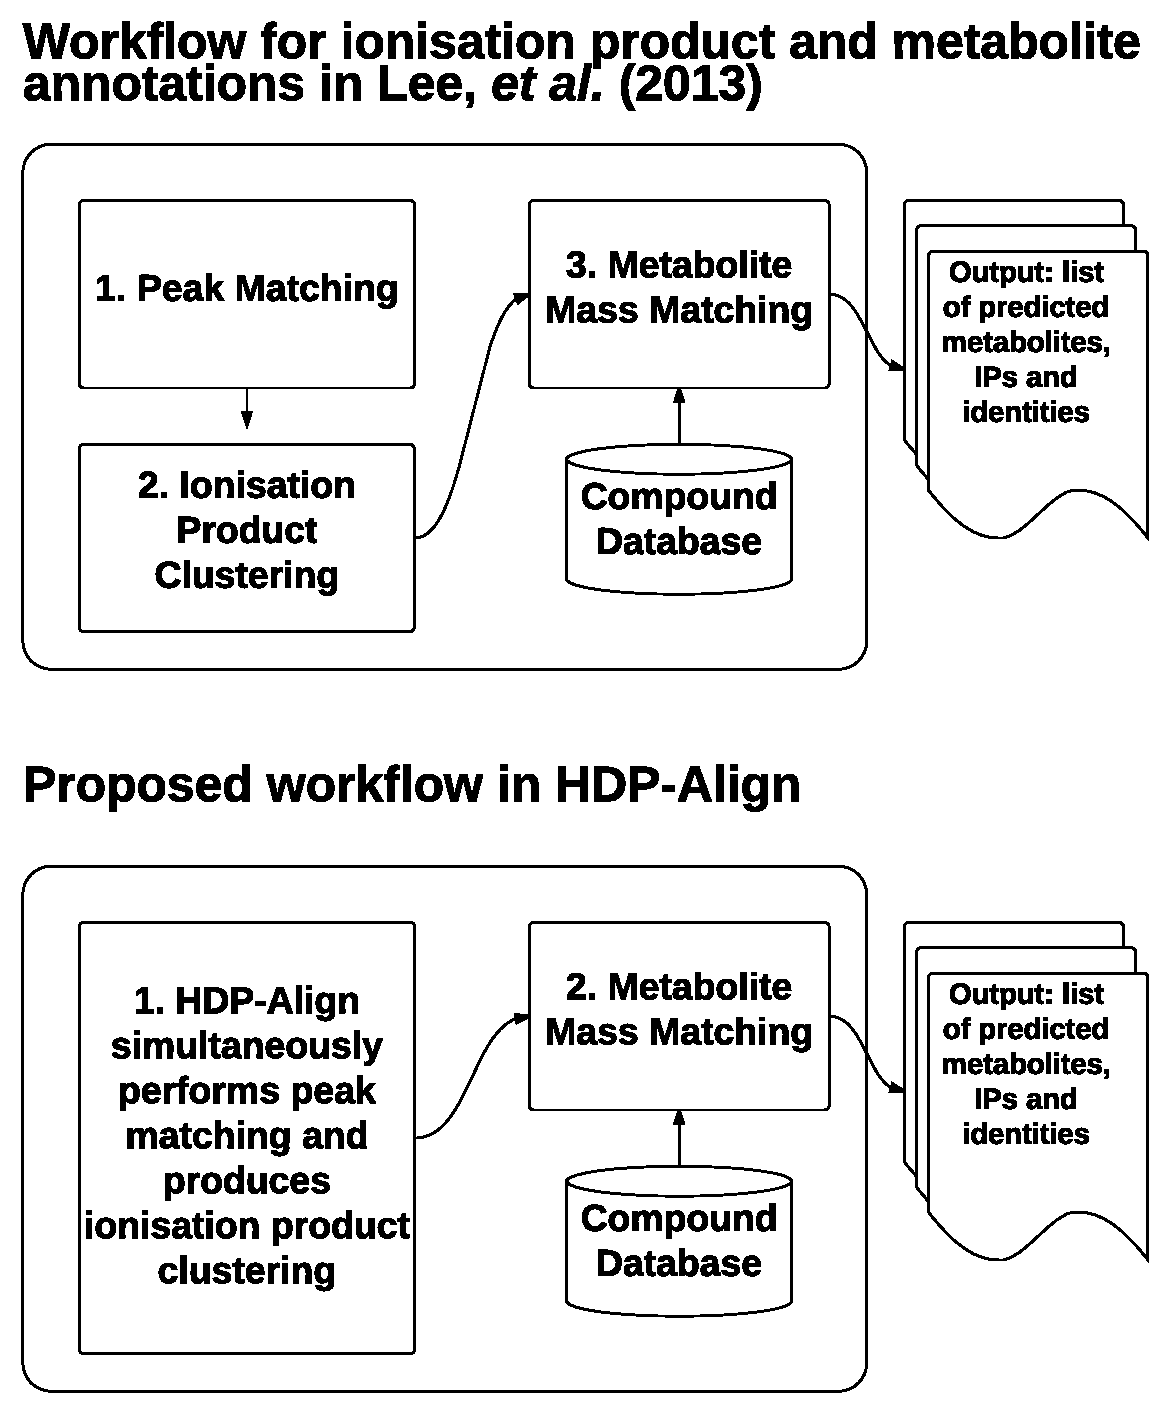
\includegraphics[width=0.7\linewidth]{06-hdp/figures/figure_3.eps}
\centering\caption{Comparisons on the workflow to assign putative annotations on isotopic products and metabolites described in \cite{Lee2013} and in HDP-Align.\label{fig-workflow}}
\end{figure}

\section{Evaluation Study}

\subsection{Evaluation Datasets}
\label{sub:Evaluation-datasets}

Performance of the proposed methods and other benchmark methods is evaluated on the LC-MS datasets of proteomic, glycomic and metabolomic experiments first introduced in Section~\ref{sub:evaluation-study}. As before, all 6 fractions from the P1 Proteomic dataset in \cite{Lange2008} are used. Each fraction contains 2 runs of features having high \ac{RT} variations across runs are used in our experiments. Unlike Section~\ref{glycomic-dataset} where only pairs of runs used, here we use the first 10 runs of the Glycomic dataset provided by \cite{Tsai2013a} for our multiple-runs experiment. Additionally, the Standard metabolomic dataset, first introduced in Section~\ref{metabolomic-dataset}, is also used. Here, we selected 6 runs for our experiment.  Table~\ref{tab:hdp-datasets} summarises the different evaluation datasets and the number of features each has.

\begin{table}[!htbp]
\begin{centering}
\begin{tabular}{|c|c|c|}
\hline 
Dataset & No. runs & Total Features\tabularnewline
\hline 
\hline 
P1 Frac 000 & 2 & 10606\tabularnewline
\hline 
P1 Frac 020 & 2 & 2135\tabularnewline
\hline 
P1 Frac 040 & 2 & 2188\tabularnewline
\hline 
P1 Frac 060 & 2 & 3342\tabularnewline
\hline 
P1 Frac 080 & 2 & 2086\tabularnewline
\hline 
P1 Frac 100 & 2 & 1326\tabularnewline
\hline 
Glycomic & 10 & 9344\tabularnewline
\hline 
Metabolomic & 6 & 7477\tabularnewline
\hline 
\end{tabular}
\par\end{centering}

\caption{Total number of runs and features of the selected evaluation datasets. \label{tab:hdp-datasets}}
\end{table}

\subsection{Performance Measures}
\label{sub:Performance-Measures}

While a definition of precision and recall in the context of alignment performance has been proposed and used in Chapter~\ref{c:matching}, the performance measures defined there applies only to pairwise alignment, i.e. an aligned peakset can only consist of two matched peak features, at most. Here, we propose a generalisation of the performance measures defined in Section~\ref{sub:experimental-setup} to apply to the alignment of multiple runs.

To provide a definition of `precision' and `recall' suitable for evaluating alignment performance of multiple runs, we first enumerate all the possible $q$-size combinations for every aligned peakset in both the method's output and the ground truth list. For example, an alignment method returns a list of two aligned peaksets $\{a,b,c,d,\},\allowbreak\{e,f,g\}$ as output. When $q=2$, this output can be enumerated into a list of 9 `alignment items' of all the pairwise combinations of features: $\{a,b\},\allowbreak\{a,c\},\allowbreak\{a,d\},\allowbreak\{b,c\},\allowbreak\{b,d\},\allowbreak\{c,d\},\allowbreak\{e,f\},\allowbreak\{e,g\},\allowbreak\{f,g\}$. Let $M$ and $G$ be the results from such enumeration from a method's output and the ground truth respectively. Each distinct combination of features in $M$ and $G$ can be considered as an item during performance evaluation. Intuitively, the choice of $q$ reflects the strictness of what is considered to be a true positive item, with larger values of $q$ demanding an alignment method that produces results spanning more runs correctly. 

For a given $q$, the following positive and negative instances of alignment item can now be defined for the purpose of performance evaluation:

\begin{itemize}
\item True Positive ($\boldsymbol{TP}$): items that should be aligned (present in $G$) and are aligned (present in $M$).
\item False Positive ($\boldsymbol{FP}$): items that should not be aligned (absent from $G$) but are aligned (present in $M$).
\item True Negative ($\boldsymbol{TN}$): items that should not be aligned (absent from $G$) and are not aligned (absent from $M$).
\item False Negative ($\boldsymbol{FN}$): items that should be aligned (present in $G$) but are not aligned (absent from $M$).
\end{itemize}

In the context of alignment performance, precision ($\frac{\boldsymbol{TP}}{\boldsymbol{TP}+\boldsymbol{FP}}$) is therefore the fraction of items in $M$ that are correct with respect to $G$, while recall ($\frac{\boldsymbol{TP}}{\boldsymbol{TP}+\boldsymbol{FN}}$) is the fraction of items in $G$ that are aligned in $M$. A method with a perfect alignment output would have both precision and recall values of 1.0. 

\subsection{Benchmarking Method}

Following Chapter~\ref{c:matching}, we benchmark HDP-Align against two established alignment methods: SIMA \cite{Voss2011a} and MZmine2's Join Aligner \cite{Pluskal2010}. The selection of SIMA and Join as the benchmark methods is motivated by the fact that both methods are direct matching methods (thus easily comparable to HDP-Align) but still differ sufficiently in how they establish the final alignment results, in particular when it comes to the alignment of multiple runs. This is primarily due to the differences between both methods in the form of the distance/similarity function between peak features, the actual matching algorithm itself and the merging order of pairwise results to construct the full alignment results.

The two most important parameters to configure in both methods are the mass and \ac{RT} tolerance parameters, used for thresholding and computing feature similarities during matching. We label these common parameters as the $T_{(m/z)}$ and $T_{rt}$ parameters. Note that despite the common label, each method may use the parameter values differently during the alignment process. In our experiments, we let $T_{(m/z)}$ and $T_{rt}$ vary within reasonable ranges (details in Section~\ref{sub:parameter-optimisations}) and report all performance values generated by each combination of the two parameters.

\subsection{Parameter Optimisations}
\label{sub:parameter-optimisations}

Tables~\ref{tab:hdp-parameters-hdpalign} and ~\ref{tab:hdp-parameters-benchmark} describe the parameter ranges of each method during performance evaluation. For HDP-Align (Table~\ref{tab:hdp-parameters-hdpalign}), we perform the experiments based on our initial choices on the appropriate parameter values. These are almost certainly less than optimal and can be optimised further. The mass cluster standard deviation $\sqrt{\rho^{-1}}$ for HDP-ALign is set to the equivalent value in parts-per-million (ppm). These are 500 ppm for the Proteomic dataset and 3 ppm for the Glycomic and Metabolomic datasets. The local (within-run) cluster \ac{RT} standard deviation $\sqrt{\gamma^{-1}}$ is assumed to be fairly constant and set to 2 seconds for all datasets, while the global cluster standard deviation $\sqrt{\delta^{-1}}$ is set in the following dataset-specific manner: 50 seconds for the Proteomic dataset and 20 seconds for the remaining datasets. The larger standard deviation value is required for the Proteomic dataset to accomodate for greater \ac{RT} drifts across runs. Other hyperparameters in HDP-Align are fixed to the following values: $\alpha'=10$, $\alpha_t=10$, $\alpha_m=100$. The values of the precision hyperparameters for global cluster RT ($\sigma_0$) and mass cluster ($\rho_0$) are set to a broad value of 1/5E6. No significant changes were found to the results when these hyperparameters for the DP concentrations and cluster precisions were varied. The mean hyperparameters $\mu_0$ and $\psi_0$ are set to the means of the RT and m/z values of the input data respectively. During inference for the Glycomic and Metabolomic datasets, 500 posterior samples were collected for the Gibbs sampling procedure, discarding the first 500 during the burn-in period. For the Proteomic dataset with larger RT deviations, 5000 posterior samples were obtained after discarding the first 5000 samples during burn-in. The number of samples is selected to ensure convergence during inference.

\begin{table}[!htbp]
\begin{centering}
\begin{tabular}{|c|c|}
\hline 
Dataset & HDP\tabularnewline
\hline 
\hline 
P1 Frac 000 & \multirow{6}{*}{$\sqrt{\rho^{-1}}=500$ ppm, $\sqrt{\gamma^{-1}}=2$ s, $\sqrt{\delta^{-1}}=50$
s}\tabularnewline
\cline{1-1} 
P1 Frac 020 & \tabularnewline
\cline{1-1} 
P1 Frac 040 & \tabularnewline
\cline{1-1} 
P1 Frac 060 & \tabularnewline
\cline{1-1} 
P1 Frac 080 & \tabularnewline
\cline{1-1} 
P1 Frac 100 & \tabularnewline
\hline 
Glycomic & $\sqrt{\rho^{-1}}=3$ ppm, $\sqrt{\gamma^{-1}}=2$ s, $\sqrt{\delta^{-1}}=20$
s\tabularnewline
\hline 
Metabolomic & $\sqrt{\rho^{-1}}=3$ ppm, $\sqrt{\gamma^{-1}}=2$ s, $\sqrt{\delta^{-1}}=20$
s\tabularnewline
\hline 
\end{tabular}
\par\end{centering}
\caption{Parameters used for HDP-Align\label{tab:hdp-parameters-hdpalign}}
\end{table}

For SIMA and Join, we report the results from all combinations of the mass and RT tolerance parameters within reasonable ranges listed in Table~\ref{tab:hdp-parameters-benchmark}. This follows from the range of parameters selected for evaluation experiments in the previous Chapter~\ref{c:matching}. The ranges of $T_{(m/z)}$ and $T_{rt}$ parameters used are based values reported on \cite{Lange2008} for the Proteomic dataset and \cite{Tsai2013a} for the Glycomic dataset. For the Metabolomic dataset, they were chosen in light of the mass accuracy and RT deviations of the data.

\begin{table}[!htbp]
\begin{centering}
\begin{tabular}{|c|c|}
\hline 
Dataset & Benchmark (SIMA, Join)\tabularnewline
\hline 
\hline 
P1 Frac 000 & \multirow{6}{*}{$T_{(m/z)}=\{1.0,1.1,...,2.0\}$, $T{}_{rt}=\{10,20,...,180\}$ s}\tabularnewline
\cline{1-1} 
P1 Frac 020 & \tabularnewline
\cline{1-1} 
P1 Frac 040 & \tabularnewline
\cline{1-1} 
P1 Frac 060 & \tabularnewline
\cline{1-1} 
P1 Frac 080 & \tabularnewline
\cline{1-1} 
P1 Frac 100 & \tabularnewline
\hline 
Glycomic & $T_{(m/z)}=\{0.05,0.1,0.25\}$,$T{}_{rt}=\{5,10,...,120\}$ s\tabularnewline
\hline 
Metabolomic & $T_{(m/z)}=\{0.001,0.01,0.1\}$, $T{}_{rt}=\{5,10,...,120\}$ s\tabularnewline
\hline 
\end{tabular}
\par\end{centering}
\caption{Parameters used for the benchmark methods (SIMA, Join).\label{tab:hdp-parameters-benchmark}}
\end{table}

\section{Results}

Precision and recall values for the evaluated methods methods on the different datasets are shown in Sections~\ref{sub:proteomic-results} and ~\ref{sub:glycomic-metabolomic-results}. Additionally, an example of the further annotations for the putative adduct type and metabolite identity that can be produced by HDP-Align is also shown in Section~\ref{sub:glycomic-metabolomic-results}. Running time of the evaluated methods are reported in Section~\ref{sub:running-time}.

\subsection{Proteomic (P1) Results}
\label{sub:proteomic-results}

Figure~\ref{fig:proteomic_results} shows the results from performance evaluation on the Proteomic (P1) dataset. We see that both benchmark methods (SIMA and Join) produce a wide range of performance depending on the parameter values for $(T_{(m/z)}, T_{rt})$ chosen. Sensitivity to parameter values is expected on this dataset due to the low mass accuracy in the MS instrument that produces the data and the high \ac{RT} drifts present across runs (further details in \cite{Lange2008}). HDP-Align performs well on several fractions (particularly fractions 040, 060, 080, 100) with precision-recall performance close to the optimal performance attainable by the benchmark methods. On all fractions, HDP-Align is also able to produce higher-precision results compared to the benchmark methods by reducing recall through setting the appropriate values for the threshold $t$. The primary benefits of quantifying alignment uncertainties is realised here as the well-calibrated probability scores on the matching confidence of aligned peak features produced HDP-Align allows the user to choose which point along the PR curve to operate on. It is less obvious how this can be accomplished in the benchmark methods by varying the \ac{RT} ($T_{rt}$) and m/z ($T_{m/z}$) thresholding parameters, if at all possible.

\begin{figure}[!htbp]
\centering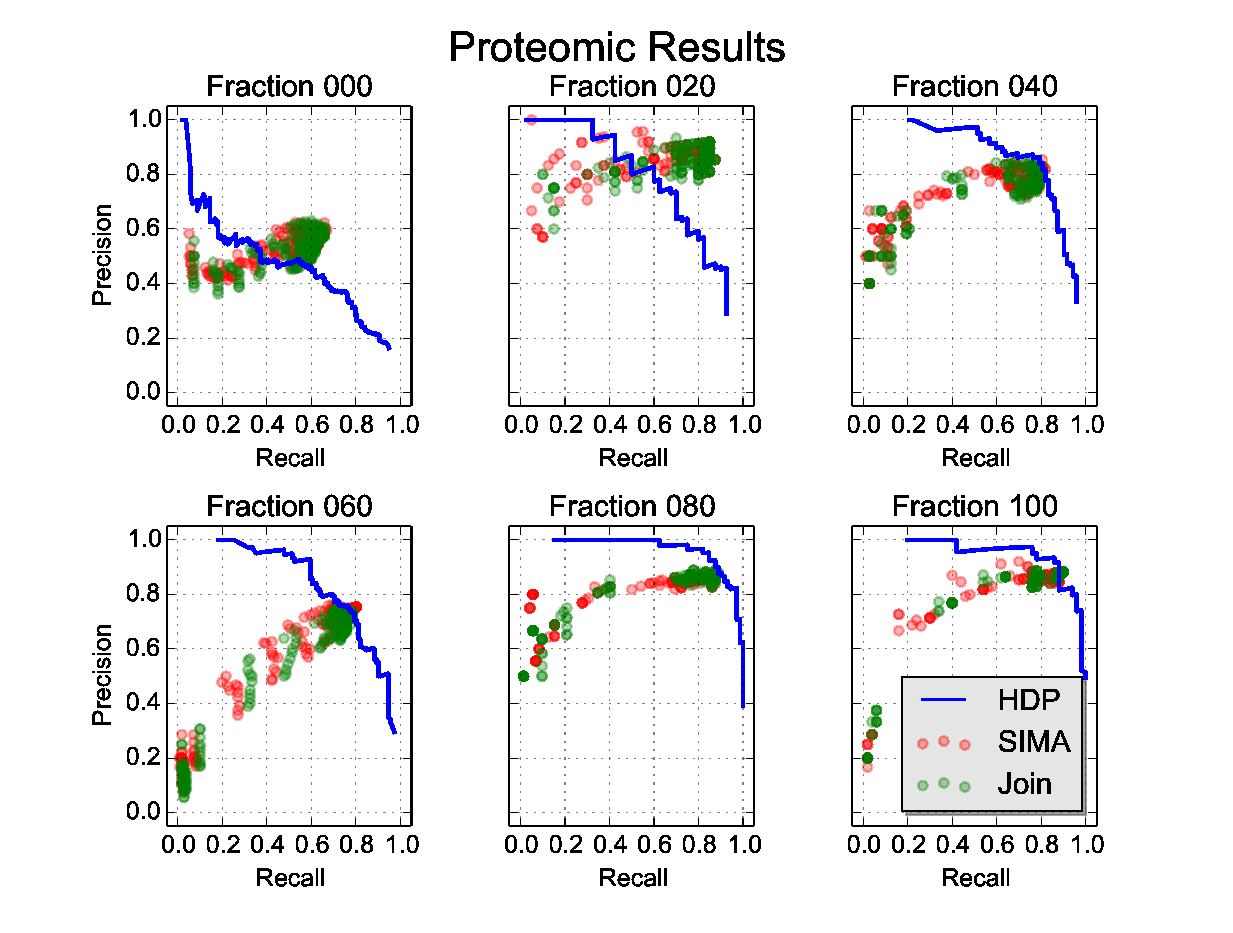
\includegraphics[width=0.7\linewidth]{06-hdp/figures/figure_4.eps}
\centering\caption{\label{fig:proteomic_results}Precision-recall values on the different fractions of the Proteomic (P1) dataset.}
\end{figure}

\subsection{Glycomic and Metabolomic Results}
\label{sub:glycomic-metabolomic-results}

Figures~\ref{fig:glycomic_results} and ~\ref{fig:metabolomic_results_alignment} show the results from experiments on the Glycomic and Metabolomic datasets. Similar to the Proteomic dataset, a wide range of precision-recall values can be observed in the results for the benchmark methods on the two datasets. The performance of HDP-Align, using the same set of parameters on both datasets, come close to the optimal results from the benchmark methods, while still allowing the user to control the desired point along the precision-recall curve to operate on.

The results for the Glycomic dataset (Figure~\ref{fig:glycomic_results}) also show some additional results on how the measured precision-recall values might change depending on the strictness of what constitutes an `item' during performance evaluation. This is accomplished by gradually increasing the value for $q$ (described in detail in Section~\ref{sub:Performance-Measures}) that determines the size of the feature combinations enumerated from a method's output. For example, $q$=2 considers all pairwise combinations of features from the method's output during performance evaluation, while $q=4$ considers all combinations of size 4, and so on. Figure~\ref{fig:glycomic_results} shows that as $q$ is increased, parameter sensitivity seems to become more of an issue for the benchmark methods, with more parameter sets having lower precisions in the results. Across all $q$s evaluated, parameter pairs that produce the best alignment performance (points with high precision and recall values) are generally small $T_{(m/z)}$ and large $T_{rt}$ values. Examples of parameter pairs that produce the best and worse performance for SIMA are shown in Figure~\ref{fig:metabolomic_results_alignment}. The results here appear to suggest the importance of having high mass precision during matching. Importantly, we see from Figure~\ref{fig:glycomic_results} that the performance of HDP-Align remains fairly consistent as $q$ is increased.

The Metabolomic dataset also provides us with additional results in form of annotations of putative adduct type and metabolite identities. A thorough evaluation on the quality of such annotations, in comparison to e.g. the workflow proposed in \cite{Lee2013}, is beyond the scope of this chapter and would likely necessitate using a different and more appropriate evaluation dataset. Instead, we present an example of the further analysis performed by HDP-Align (as proposed in Section~\ref{subsub:isotopic-product-annotations}) on the resulting clustering objects after inference. Figure~\ref{fig:metabolomic_results_annotations} shows a global \ac{RT} cluster where peak features across runs have been grouped by their \ac{RT} and m/z values. Within this global cluster, peak features are further separated into 6 mass clusters -- corresponding to ionisation products produced by the global cluster during mass spectometry. In Figure~\ref{fig:metabolomic_results_annotations}, mass cluster $A$ and $B$ contain features aligned from several runs but they do not have any other mass cluster sharing a possible precursor mass. Mass cluster $C$ and $D$ share a common precursor mass (292.12696) and can thus be annotated by the adduct type that produce the transformation. Similarly, mass cluster $E$ and $F$ share a common precursor mass at 383.14278. Queries to a local KEGG database are issued based on the precursor mass values, producing several compound identities that can be putatively assigned to the global \ac{RT} cluster. It is a great strength of our approach that this putative identification step appears very naturally from the alignment results.

\begin{figure}[!htbp]
\centering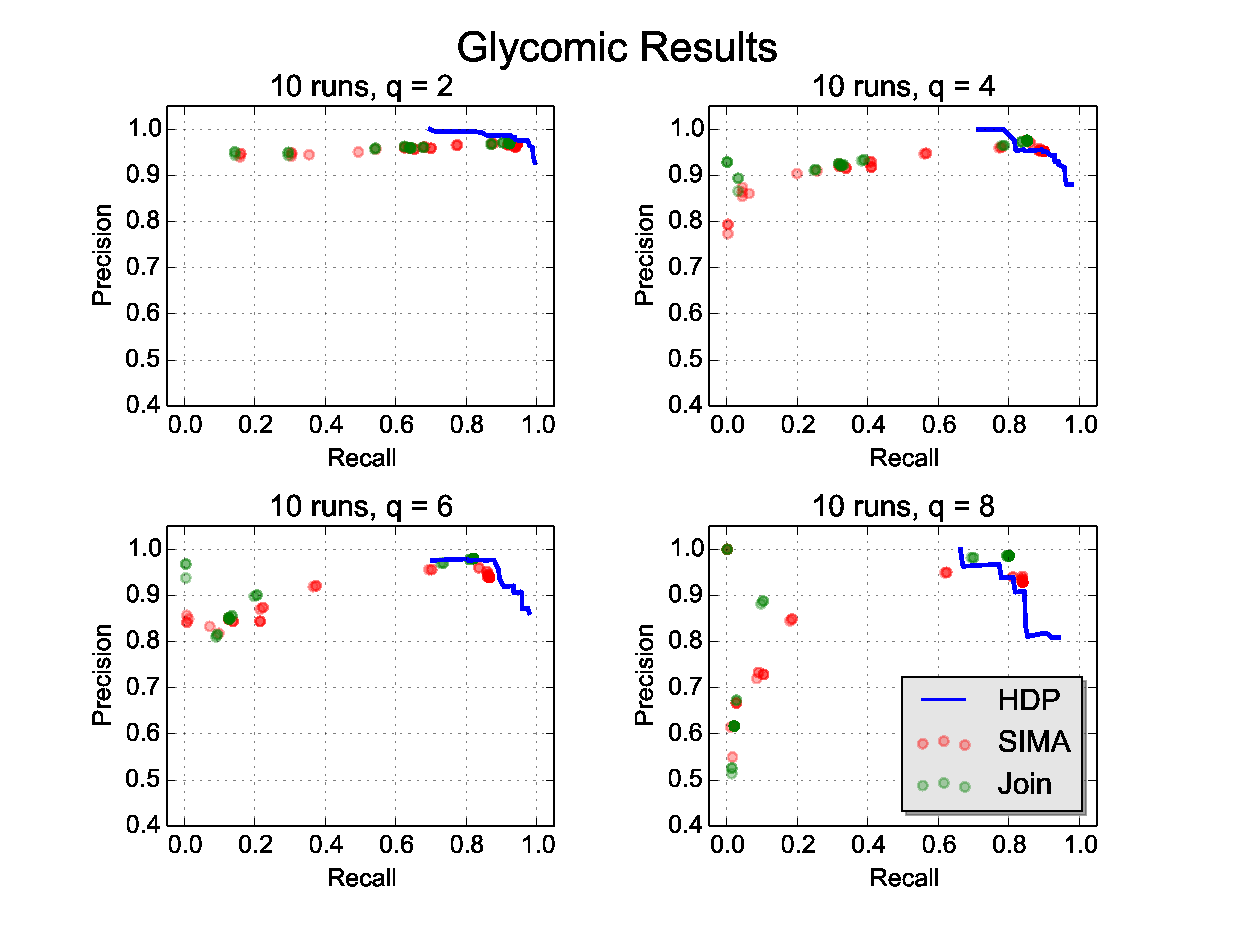
\includegraphics[width=0.7\linewidth]{06-hdp/figures/figure_5.eps}
\centering\caption{\label{fig:glycomic_results}Precision-recall values on the alignment of 10 runs from the Glycomic dataset when $q$ (the strictness of performance evaluation as described in Section~\ref{sub:Performance-Measures}) is gradually increased.}
\end{figure}

\begin{figure}[!htbp]
\centering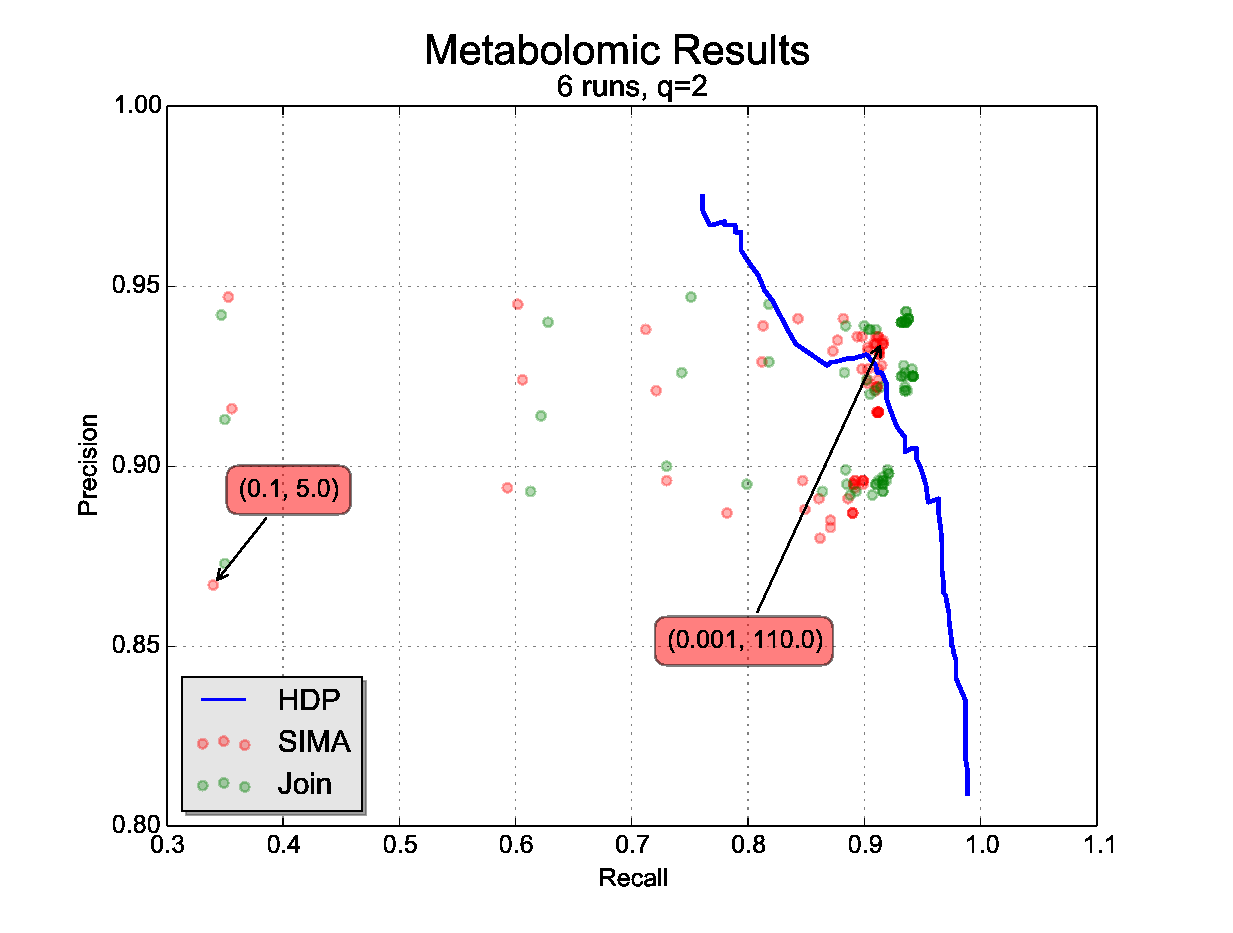
\includegraphics[width=0.7\linewidth]{06-hdp/figures/figure_6.eps}
\centering\caption{\label{fig:metabolomic_results_alignment}Precision-recall values on the alignment of 6 runs from the Metabolomic dataset. The parameter values $(T_{m/z}, T_{rt})$ that produce the best and worst performance in SIMA are also annotated in the Figure (red boxes).}
\end{figure}

\begin{figure}[!htbp]
\centering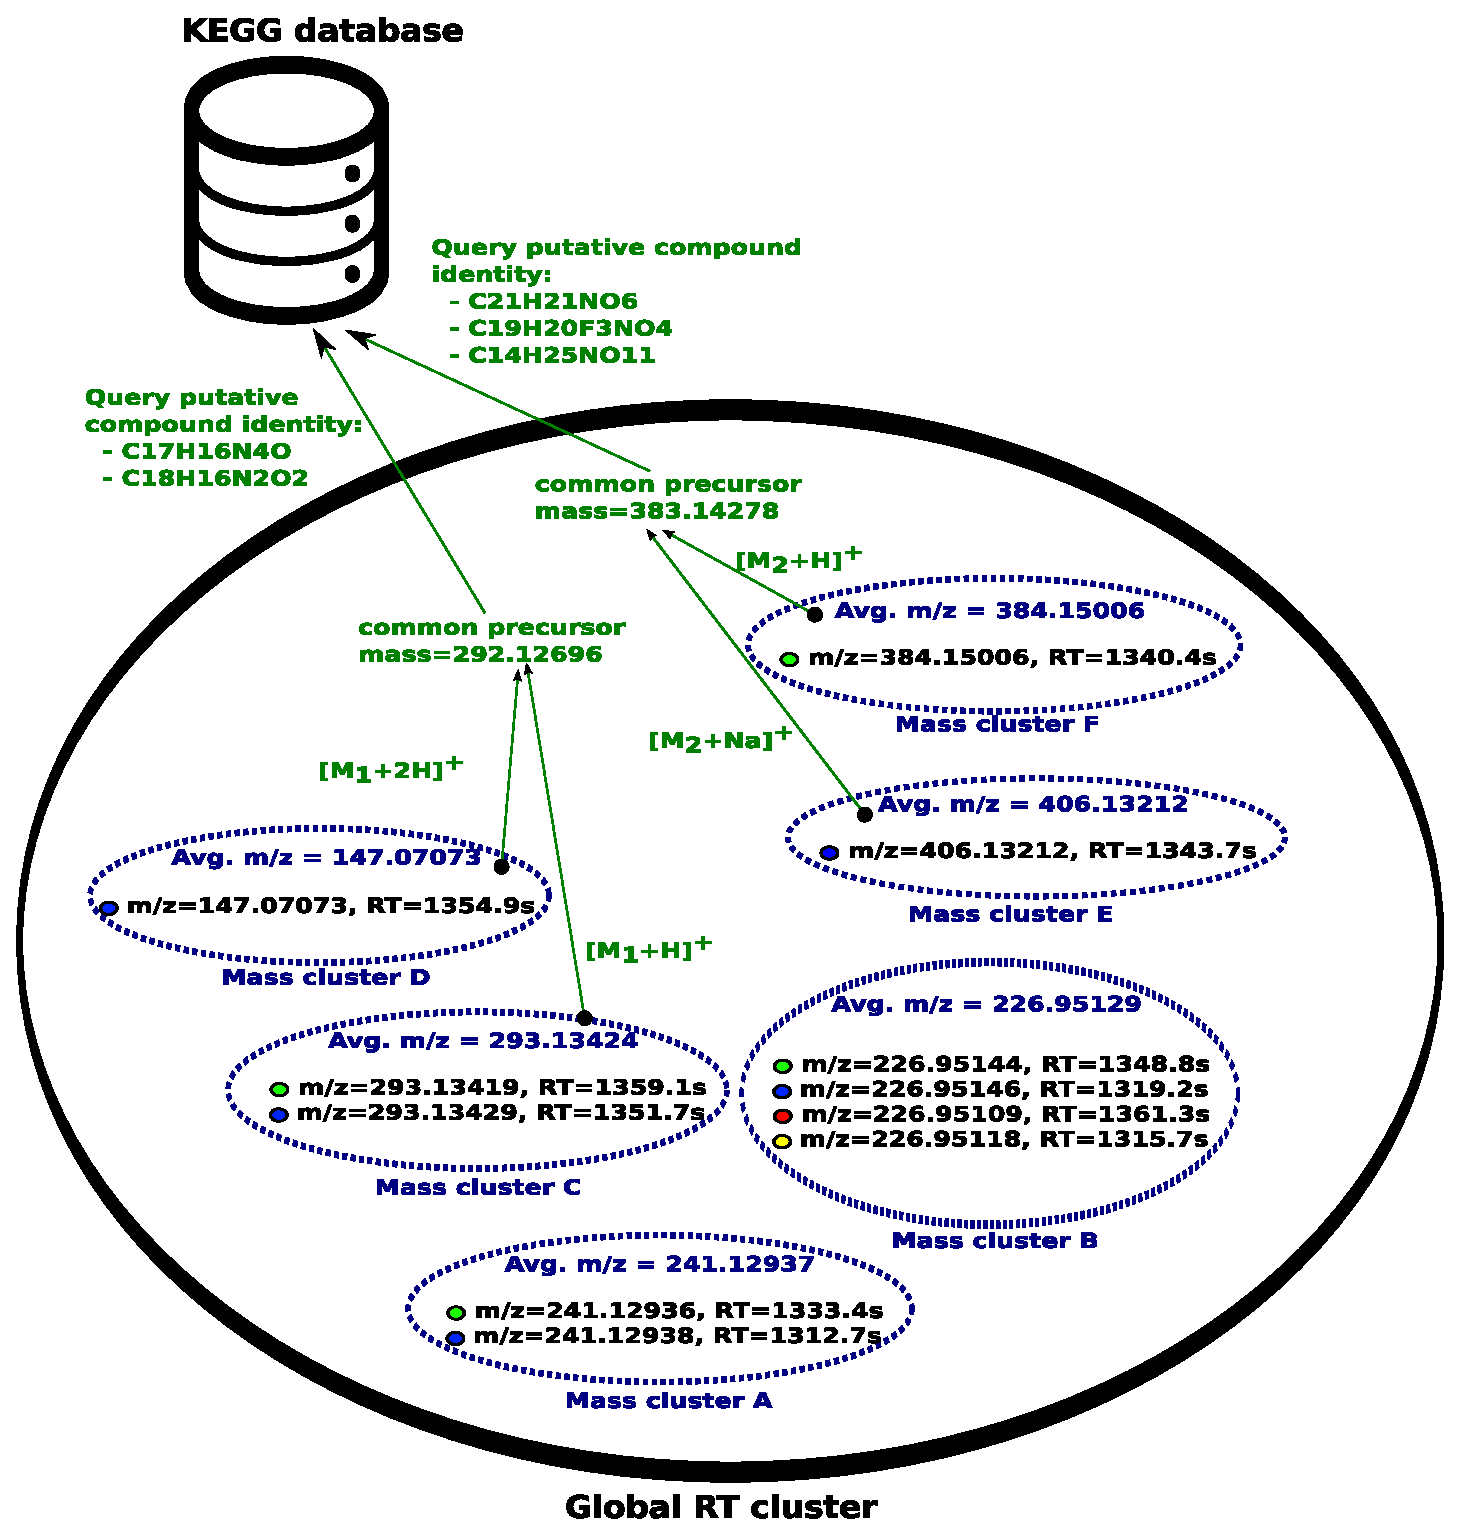
\includegraphics[width=0.7\linewidth]{06-hdp/figures/figure_7.eps}
\centering\caption{\label{fig:metabolomic_results_annotations}Example analysis that can be performed on the clustering objects inferred in a Gibbs sample from HDP-Align. The outer black oval denotes a global RT cluster (generally corresponding to a metabolite compound), while the smaller dotted ovals within denote mass clusters (labelled as mass cluster $A,B,C,D,E,F$). Peak features are denoted by the filled circle, with the fill colour indicating the originating run of a peak. Green colours denote additional analysis steps that can be performed on the mass cluster objects. \textbf{REDRAW TO LOOK NICER?}}
\end{figure}

\subsection{Running Time}
\label{sub:running-time}

The main factor affecting the running time of HDP-Align is the total number of peaks across all runs to be processed and the number of samples produced during Gibbs sampling. In each iteration of Gibbs sampling, HDP-Align removes a peak from the model, updates parameters of the model conditioned on every other parameters, and reassigns a peak into RT and mass clusters. The time complexity of this operation is $O(N)$, where $N$ is the total number of peaks across all runs. In practice, additional time will also be spent on various necessary book-keeping operations, such as deleting empty clusters that are no longer required, updating internal data structures, etc. A representative running time is given as $N=9344$ for the Glycomic dataset. HDP-Align requires approximately 5 hours to collect 1000 samples. In comparison, both SIMA and Join perform alignment within 5 to 10 seconds. Similarly, for $N=7477$ for the Metabolomic dataset, HDP-Align produces the results in approximately 4 hours after collecting 1000 samples, while SIMA and Join complete within seconds. The running time of HDP-Align, while being significantly longer than these two benchmark methods, is comparable to other computationally-intensive steps (e.g. peak detection) in a typical LC-MS pipeline.

\section{Discussion and Conclusion}

\label{sec:conc}

We have presented a hierarchical non-parametric Bayesian model that performs direct matching of peak features, a problem of significant importance in the data pre-processing pipeline of large untargeted LC-MS datasets. Unlike other direct matching methods, the novelty of our proposed approach lies in its ability of to produce well-calibrated probability scores on the matching confidence of aligned peak features (evidenced by the increasing precision and decreasing recall as the threshold $t$ is increased). This is accomplished by casting the multiple alignment problem of LC-MS peak features as a hierarchical clustering problem. Matching confidence can then be obtained based on the probabilities of co-eluting peak features to be assigned under the same mass component of the same global cluster. Experiments based on datasets from real proteomic, glycomic and metabolomic experiments show that HDP-Align is able to produce alignment results competitive to the benchmark alignment methods, with the added benefit of being able to provide a measure of confidence in the alignment quality. This can be useful in real analytical situations, where neither the optimal parameters nor the alignment ground truth is known to the user.

Through comparisons against benchmark methods, our studies have also investigated the effect of sub-optimal parameter choices on alignment performance. While beyond the scope of our paper, we agree with \cite{Smith2013, Smith2013a} that thorough investigations into the influence of numerous configurable parameters (prevalent in nearly all LC-MS data processing pipeline) on the resulting biological conclusions are of utmost importance. This should be followed by the development of methods to minimise or automatically-tune such configurable parameters. Despite the abundance of new methods proposed for LC-MS data pre-processing, relatively few studies have been done on the subject of quantifying uncertainties and alleviating the burden of parameter optimisations during actual data analysis. One way to minimise the number of parameters is through the integration of multiple steps in the typical LC-MS pipeline into fewer steps. Our proposed model in HDP-Align can potentially be extended in this manner, as evidenced by the metabolomic dataset results where we directly use the clustering objects inferred from the model to perform further analysis on putative adduct and metabolite type annotations. While the proposed annotation approach in Section~\ref{subsub:isotopic-product-annotations} is fairly simple, it can be easily extended to more sophisticated annotation strategies, such as in CAMERA \cite{Kuhl2012}. 

A primary weakness of HDP-Align lies in the long computational time required to produce results. Additional work will be required to reduce the computational burden of the model through various optimisation tricks and potentially by parallelising the Gibbs inference step using e.g. the method described in \cite{Lovell2012}. Another possibility is to adopt a different non-sampling-based inferential approach or perhaps even a simpler model altogether, while still retaining the essence and benefits of the HDP-Align model. The key insight here lies in modelling related peaks as within-file clusters in a single run but also allowing these within-file clusters to be generated by globally-shared clusters spanning across multiple runs. The results presented in the current chapter suggest the method shows enough promise to warrant the effort to speed it up, and indeed that is what we will discuss in the next chapter.

Another aspect worthy of investigation is determining the most effective way to present and visualise the alignment probabilities produced by HDP-Align. Additional sources of information present in the LC-MS data, such as chromatographic peak shapes, can also be used to improve alignment performance and subsequent analyses that follow. 

Finally, replacing or enhancing the mixture of mass components used in HDP-Align with a more appropriate mass model, such as that in MetAssign \cite{Daly2014} that specifically takes into account the inter-dependency structure of peaks, is an avenue for future work. This will be particularly useful when extending the proposed model in HDP-Align into a single inferential model that encompasses many intermediate steps in a typical LC-MS data processing pipeline.